\documentclass[a4paper,12pt]{article}
\usepackage[utf8]{inputenc}
\usepackage[german]{babel}
\usepackage{amsmath}
\usepackage{amssymb}
\usepackage{amsthm}
\usepackage{geometry}
\usepackage{graphicx}
\usepackage[hidelinks]{hyperref}
\usepackage{listings}
\usepackage{xcolor}
\usepackage{enumitem}
\usepackage{booktabs}
\usepackage{array}

\geometry{margin=2.5cm}

\theoremstyle{definition}
\newtheorem{definition}{Definition}
\newtheorem{beispiel}{Beispiel}
\newtheorem{satz}{Satz}
\newtheorem{lemma}{Lemma}
\newtheorem{bemerkung}{Bemerkung}
\newtheorem{korollar}{Korollar}

\setlist[itemize,1]{label=--}

% ---------- Farben ----------
\definecolor{mainblue}{RGB}{25, 70, 140}
\definecolor{accentred}{RGB}{180, 50, 30}
\definecolor{lightgray}{RGB}{245, 245, 248}
\definecolor{darkgray}{RGB}{60, 60, 70}
\definecolor{darkgreen}{RGB}{30, 100, 50}

\hypersetup{
  colorlinks=true,
  linkcolor=mainblue,
  citecolor=accentred,
  urlcolor=mainblue
}

\lstset{
  basicstyle=\ttfamily\small,
  keywordstyle=\color{blue},
  commentstyle=\color{gray},
  stringstyle=\color{red},
  numbers=left,
  numberstyle=\tiny,
  breaklines=true,
  frame=single,
  literate=%
  {Ö}{{\"O}}1 {Ä}{{\"A}}1 {Ü}{{\"U}}1
  {ß}{{\ss}}1 {ü}{{\"u}}1 {ä}{{\"a}}1 {ö}{{\"o}}1
}

\title{Die Knotengleichung als universelles Naturgesetz\\[0.4em]
  \large Vom elektrischen Strom zum atmosphärischen Gleichgewicht der Wolkenmasse über der Erde}
\author{Stephan Epp\\[0.3em]
  
\date{7. Mai 2026}

\begin{document}

\maketitle

\begin{abstract}
Die Knotengleichung -- auch Knotenpunktsatz oder Kirchhoffsches Stromgesetz
genannt -- ist eines der fundamentalsten Prinzipien der Physik: An jedem Knoten
eines Netzes muss die Summe aller zufließenden Größen gleich der Summe aller
abfließenden Größen sein. Dieses Prinzip, formal als $\sum I_\mathrm{zu} =
\sum I_\mathrm{ab}$ geschrieben, gilt nicht nur für elektrische Ströme, sondern
ist ein universelles Erhaltungsgesetz, das überall in der Natur wirkt, wo
Massenflüsse oder Energieflüsse auftreten.

In der vorliegenden Arbeit werden zwei fundamentale Ausprägungen dieses Gesetzes
formal bewiesen und quantitativ analysiert: zunächst das Kirchhoffsche
Stromgesetz in elektrischen Netzwerken (1845), anschließend das
atmosphärisch-hydrologische Gleichgewicht der gesamten Wolkenmasse über der Erde,
beschrieben durch die Kontinuitätsgleichung für Wasserdampf. Beide Phänomene
werden in ein gemeinsames graphtheoretisches Rahmenwerk eingebettet, in dem der
Subgraph Algorithmus (Epp~2026) als Analyse\-instrument für Flussnetze eingesetzt
wird. Fünf Matplotlib-Visualisierungen illustrieren die theoretischen Ergebnisse
quantitativ.
\end{abstract}

\tableofcontents
\newpage

% ===========================================================================
\section{Einführung}
% ===========================================================================

\subsection{Problemstellung}

Die Knotengleichung, in der Elektrotechnik als Kirchhoffsches Stromgesetz
(KSG) bekannt, lautet in ihrer allgemeinsten Form:
\[
  \sum_{k=1}^{m} \phi_k = 0,
\]
wobei $\phi_k$ die $k$-te Flussgröße (Strom, Massenstrom, Volumenstrom,
Feuchtefluss, \ldots) am Knoten bezeichnet, mit dem Vorzeichen\-konvent~$+$ für
Zufluss und $-$ für Abfluss.

\textbf{Zentrale Frage dieser Arbeit:} Ist die Knotengleichung ein universelles
Naturgesetz, das sowohl für den elektrischen Strom als auch für das Gleichgewicht
der gesamten atmosphärischen Wolkenmasse über der Erde gilt, und wie lässt sich
dieser Zusammenhang formal und quantitativ nachweisen?

\subsection{Motivation}

Das Prinzip \emph{Zufluss gleich Abfluss} tritt in vielen Naturwissen\-schaften
auf. In der Elektrotechnik ist es eine unmittelbare Folge der
Ladungserhaltung~\cite{kirchhoff1845}. In der Atmosphären\-wissenschaft
manifestiert es sich als Gleichgewicht des globalen Wasserkreislaufs: Die
Gesamtverdunstung der Meere und Landmassen ($E \approx 577\,000\;\text{km}^3/\text{a}$)
muss global exakt dem Gesamtniederschlag ($P \approx 577\,000\;\text{km}^3/\text{a}$)
entsprechen~\cite{trenberth2011}, weil sonst die Masse der Atmosphäre
unbegrenzt wachsen oder schrumpfen würde -- was den Naturgesetzen widerspräche.

Der Subgraph Algorithmus (Epp~2026, $\Theta(n^3)$) \cite{epp2026} liefert
ein graphtheoretisches Modellierungs\-werkzeug, mit dem Flussnetze -- sowohl
elektrische Schaltkreise als auch das globale Flussnetz des Wasser\-kreislaufs
-- als gerichtete, gewichtete Graphen repräsentiert und analysiert werden können.

% ===========================================================================
\section{Grundlagen}
% ===========================================================================

\subsection{Mathematische Definitionen}

\begin{definition}[Flussnetz]
  Ein Flussnetz ist ein gerichteter, gewichteter Graph $G = (V, E, f)$, wobei
  $V$ die Menge der Knoten, $E \subseteq V \times V$ die Menge der gerichteten
  Kanten und $f: E \to \mathbb{R}$ eine Flussfunktion ist.
\end{definition}

\begin{definition}[Knotengleichung / Flussbilanz]
  \label{def:knotengleichung}
  Sei $G = (V, E, f)$ ein Flussnetz. Die Knotengleichung für einen Knoten
  $v \in V$ lautet:
  \[
    \sum_{u:\,(u,v)\in E} f(u,v) \;=\; \sum_{w:\,(v,w)\in E} f(v,w).
  \]
  Äquivalent in Vorzeichenform: $\displaystyle\sum_{k} \phi_k(v) = 0$, wobei
  $\phi_k(v)$ die $k$-te Flussgröße am Knoten~$v$ ist
  (positiv für Zufluss, negativ für Abfluss).
\end{definition}

\begin{definition}[Adjazenzmatrix eines Flussnetzes]
  Die gewichtete Adjazenzmatrix $A$ eines Flussnetzes $G$ mit $n$ Knoten ist
  eine $n \times n$ Matrix mit:
  \[
    A_{ij} = \begin{cases} f(v_i, v_j) & \text{falls } (v_i, v_j) \in E \\ 0 & \text{sonst.} \end{cases}
  \]
\end{definition}

\begin{definition}[Laplace-Matrix / Kirchhoff-Matrix]
  Sei $D$ die Diagonalmatrix mit $D_{ii} = \sum_j A_{ij}$ (Ausgangsgrade).
  Die Laplace-Matrix des Flussnetzes ist $L = D - A$. Die Knotengleichung
  für alle Knoten lautet kompakt:
  \[
    L \,\mathbf{f} = \mathbf{0},
  \]
  wobei $\mathbf{f}$ der Flussvektor ist.
\end{definition}

\begin{definition}[Kontinuitätsgleichung für Wasserdampf]
  Sei $\rho_w(\mathbf{x}, t)$ die spezifische Feuchte [kg/kg] und
  $\mathbf{v}(\mathbf{x}, t)$ das dreidimensionale Windfeld. Die
  Kontinuitätsgleichung für atmosphärischen Wasserdampf lautet:
  \[
    \frac{\partial \rho_w}{\partial t} + \nabla \cdot (\rho_w \mathbf{v})
    = \dot{E} - \dot{P},
  \]
  wobei $\dot{E}$ [kg\,m$^{-2}$\,s$^{-1}$] die Evaporationsrate und
  $\dot{P}$ die Niederschlagsrate ist.
\end{definition}

\subsection{Physikalische Grundprinzipien}

Beiden hier betrachteten Ausprägungen der Knotengleichung liegen
fundamentale Erhaltungssätze der Physik zugrunde:

\begin{itemize}
  \item \textbf{Elektrotechnik:} Erhaltung der elektrischen Ladung
    ($\nabla \cdot \mathbf{J} = -\partial\rho_e/\partial t$)
  \item \textbf{Atmosphäre:} Erhaltung der Wassermasse
    ($\partial\rho_w/\partial t + \nabla \cdot (\rho_w \mathbf{v}) = \dot{E} - \dot{P}$)
  \item \textbf{Allgemein:} Jedes Erhaltungsgesetz erzeugt an jedem Knoten
    eine Flussbilanz -- die Knotengleichung.
\end{itemize}

% ===========================================================================
\section{Die Knotengleichung in der Elektrotechnik}
% ===========================================================================

\subsection{Historischer Hintergrund}

Gustav Robert Kirchhoff formulierte 1845, damals noch Student in Königsberg,
seine beiden grundlegenden Sätze für elektrische Netzwerke~\cite{kirchhoff1845}.
Der erste Kirchhoffsche Satz (Knotenpunktsatz, KSG) besagt, dass sich an
jedem Knoten eines elektrischen Netzwerkes die Summe aller zufließenden
und abfließenden Ströme zu null addiert:
\[
  \sum_{k=1}^{m} I_k = 0.
\]

\subsection{Formaler Beweis des Kirchhoffschen Stromgesetzes}

\begin{satz}[Kirchhoffsches Stromgesetz, KSG]
  \label{satz:ksg}
  In einem elektrischen Netzwerk im stationären Zustand gilt an jedem
  Knoten~$v$:
  \[
    \sum_{k=1}^{m} I_k(v) = 0,
  \]
  wobei $I_k(v)$ die Stromstärke im $k$-ten Zweig am Knoten $v$ ist,
  mit $I_k > 0$ für zufließenden und $I_k < 0$ für abfließenden Strom.
\end{satz}

\begin{proof}
  \textbf{Schritt~1: Ladungserhaltung (Maxwell).}\\
  Aus dem Maxwellschen Gleichungssystem folgt die Kontinuitätsgleichung
  für elektrische Ladung:
  \[
    \nabla \cdot \mathbf{J} = -\frac{\partial \rho_e}{\partial t},
  \]
  wobei $\mathbf{J}$ [A/m$^2$] die elektrische Stromdichte und $\rho_e$
  [C/m$^3$] die Raumladungsdichte ist.

  \textbf{Schritt~2: Stationärer Zustand.}\\
  Im stationären Zustand gilt $\partial \rho_e / \partial t = 0$, also:
  \[
    \nabla \cdot \mathbf{J} = 0.
  \]

  \textbf{Schritt~3: Integration über ein Kontrollvolumen.}\\
  Sei $V_v$ ein kleines Kontrollvolumen um Knoten $v$ mit Oberfläche
  $\partial V_v$. Integration der Divergenzgleichung über $V_v$:
  \[
    \int_{V_v} \nabla \cdot \mathbf{J}\, \mathrm{d}V = 0.
  \]

  \textbf{Schritt~4: Gaußscher Integralsatz.}\\
  Der Gaußsche Integralsatz liefert:
  \[
    \oint_{\partial V_v} \mathbf{J} \cdot \mathrm{d}\mathbf{A} = 0.
  \]
  Das Oberflächenintegral über $\partial V_v$ zerfällt in die Beiträge
  der $m$ an Knoten $v$ angeschlossenen Zweige. Für Zweig $k$ gilt:
  \[
    \int_{A_k} \mathbf{J} \cdot \mathrm{d}\mathbf{A} = I_k(v).
  \]

  \textbf{Schritt~5: Knotengleichung.}\\
  Damit folgt unmittelbar:
  \[
    \sum_{k=1}^{m} I_k(v) = \oint_{\partial V_v} \mathbf{J} \cdot \mathrm{d}\mathbf{A} = 0. \qedhere
  \]
\end{proof}

\begin{lemma}[Eindeutigkeit der Stationärität]
  \label{lem:stationaer}
  Im stationären Zustand ist die Verletzung der Knotengleichung an einem
  Knoten~$v$ mit Ausmaß $\varepsilon > 0$ physikalisch unmöglich, da sonst
  $\partial \rho_e / \partial t = \varepsilon / V_v \neq 0$ gelten würde, was
  dem angenommenen stationären Zustand widerspricht.
\end{lemma}

\begin{proof}
  Angenommen, $\sum_k I_k(v) = \varepsilon \neq 0$. Dann gilt nach
  Schritt~3--4 des Beweises von Satz~\ref{satz:ksg}:
  \[
    \int_{V_v} \nabla \cdot \mathbf{J}\, \mathrm{d}V = \varepsilon \neq 0.
  \]
  Aus der Kontinuitätsgleichung folgt dann
  $-\int_{V_v} \partial\rho_e/\partial t\, \mathrm{d}V = \varepsilon$,
  also akkumuliert sich Ladung bei Knoten~$v$ mit Rate $\varepsilon/V_v$.
  Dies widerspricht der Stationaritätsbedingung. Widerspruch. \qedhere
\end{proof}

\subsection{Quantitatives Beispiel}

\begin{beispiel}[Elektrischer Knoten mit sechs Zweigen]
  Gegeben sei ein Knoten $K$ mit sechs angeschlossenen Zweigen (vgl.
  Abbildung~\ref{fig:kirchhoff}):
  \[
    I_1 = +4\,\text{A},\quad I_2 = +2\,\text{A},\quad I_3 = +1\,\text{A},
  \]
  \[
    I_4 = -3\,\text{A},\quad I_5 = -2\,\text{A},\quad I_6 = -2\,\text{A}.
  \]
  Prüfung der Knotengleichung:
  \[
    \sum_{k=1}^{6} I_k = 4 + 2 + 1 - 3 - 2 - 2 = 0. \qquad \checkmark
  \]
  Zustrom: $4 + 2 + 1 = 7\,\text{A}$, Abstrom: $3 + 2 + 2 = 7\,\text{A}$.
\end{beispiel}

\begin{figure}[h]
  \centering
  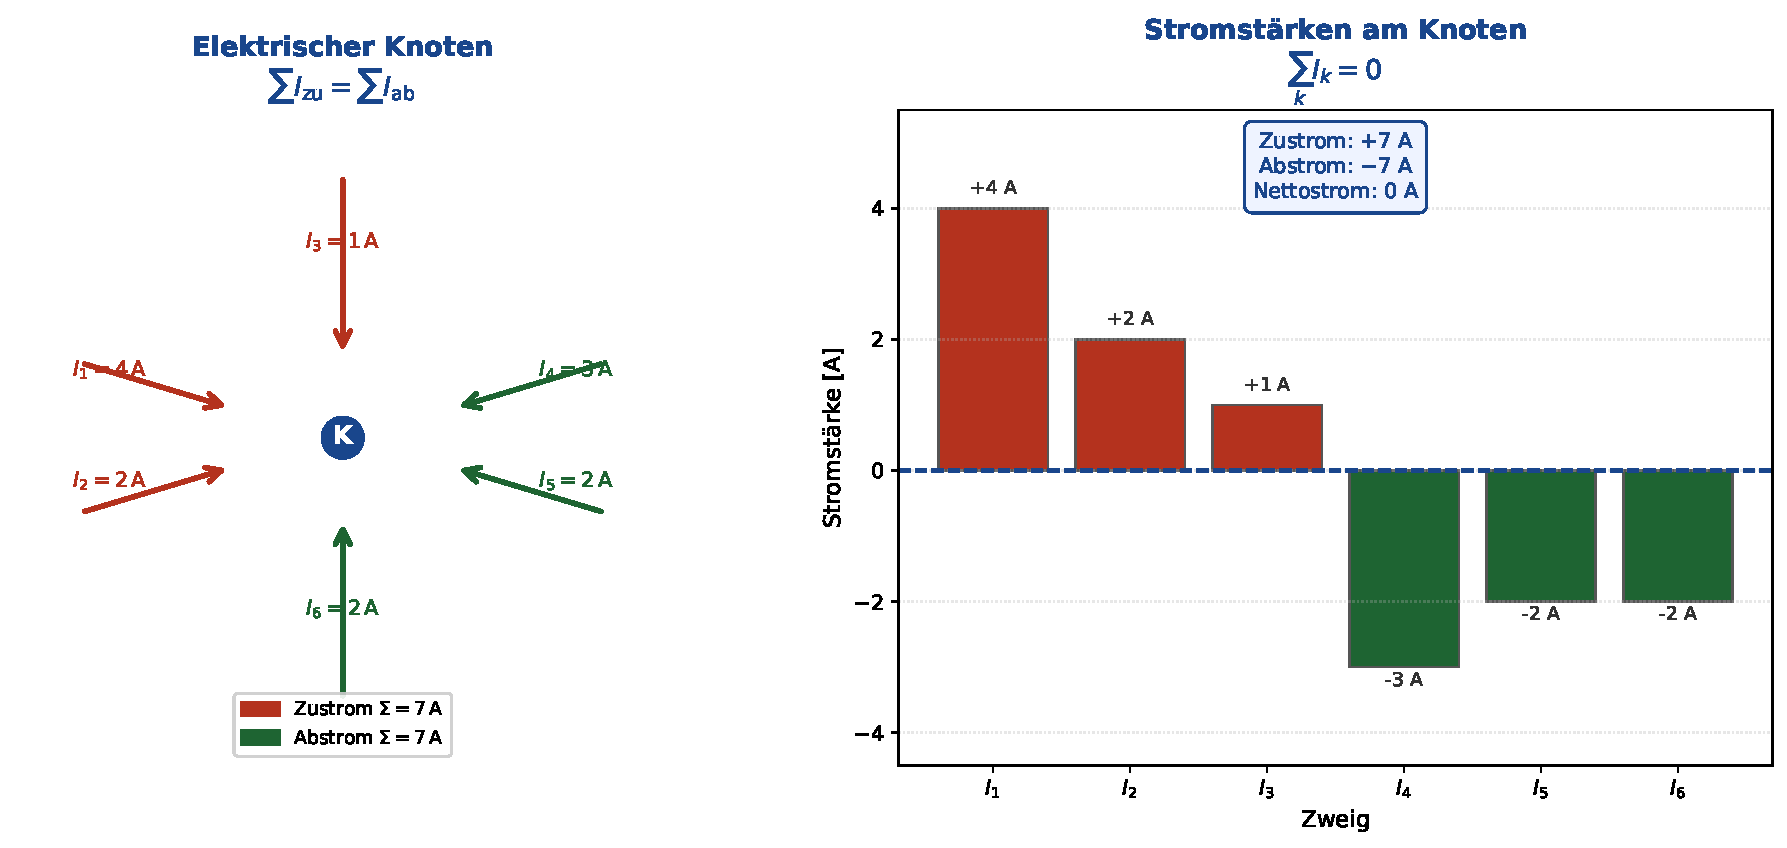
\includegraphics[width=\textwidth]{plot1_kirchhoff.pdf}
  \caption{Kirchhoffscher Knotendiagramm: Links das Knotendiagramm mit
    Stromrichtungen (rot: Zustrom, grün: Abstrom), rechts die Balkendar\-stellung
    der Stromstärken. Die Summe aller Ströme ergibt exakt null
    ($\sum I_k = 0$). Eigene Darstellung.}
  \label{fig:kirchhoff}
\end{figure}

% ===========================================================================
\section{Die Knotengleichung in der Atmosphäre}
% ===========================================================================

\subsection{Das atmosphärische Flussnetz der Erde}

Die Erde bildet ein geschlossenes thermodynamisches System (im
Sinne des Massentransports). Die gesamte atmosphärische Wolkenmasse
und der Wasserdampf befinden sich in einem dynamischen Gleichgewicht:
\begin{itemize}
  \item Von den Ozeanen und Landmassen verdunstet pro Jahr eine
    Gesamtwassermenge von $E_\mathrm{global} \approx 577\,000\;\text{km}^3$
    \cite{trenberth2011}.
  \item Als Niederschlag (Regen, Schnee, Tau) fallen global pro Jahr
    $P_\mathrm{global} \approx 577\,000\;\text{km}^3$ aus.
  \item Die Differenz $E_\mathrm{global} - P_\mathrm{global} = 0$ ist
    Ausdruck der atmosphärischen Knotengleichung auf der Globalskala.
\end{itemize}

\begin{figure}[h]
  \centering
  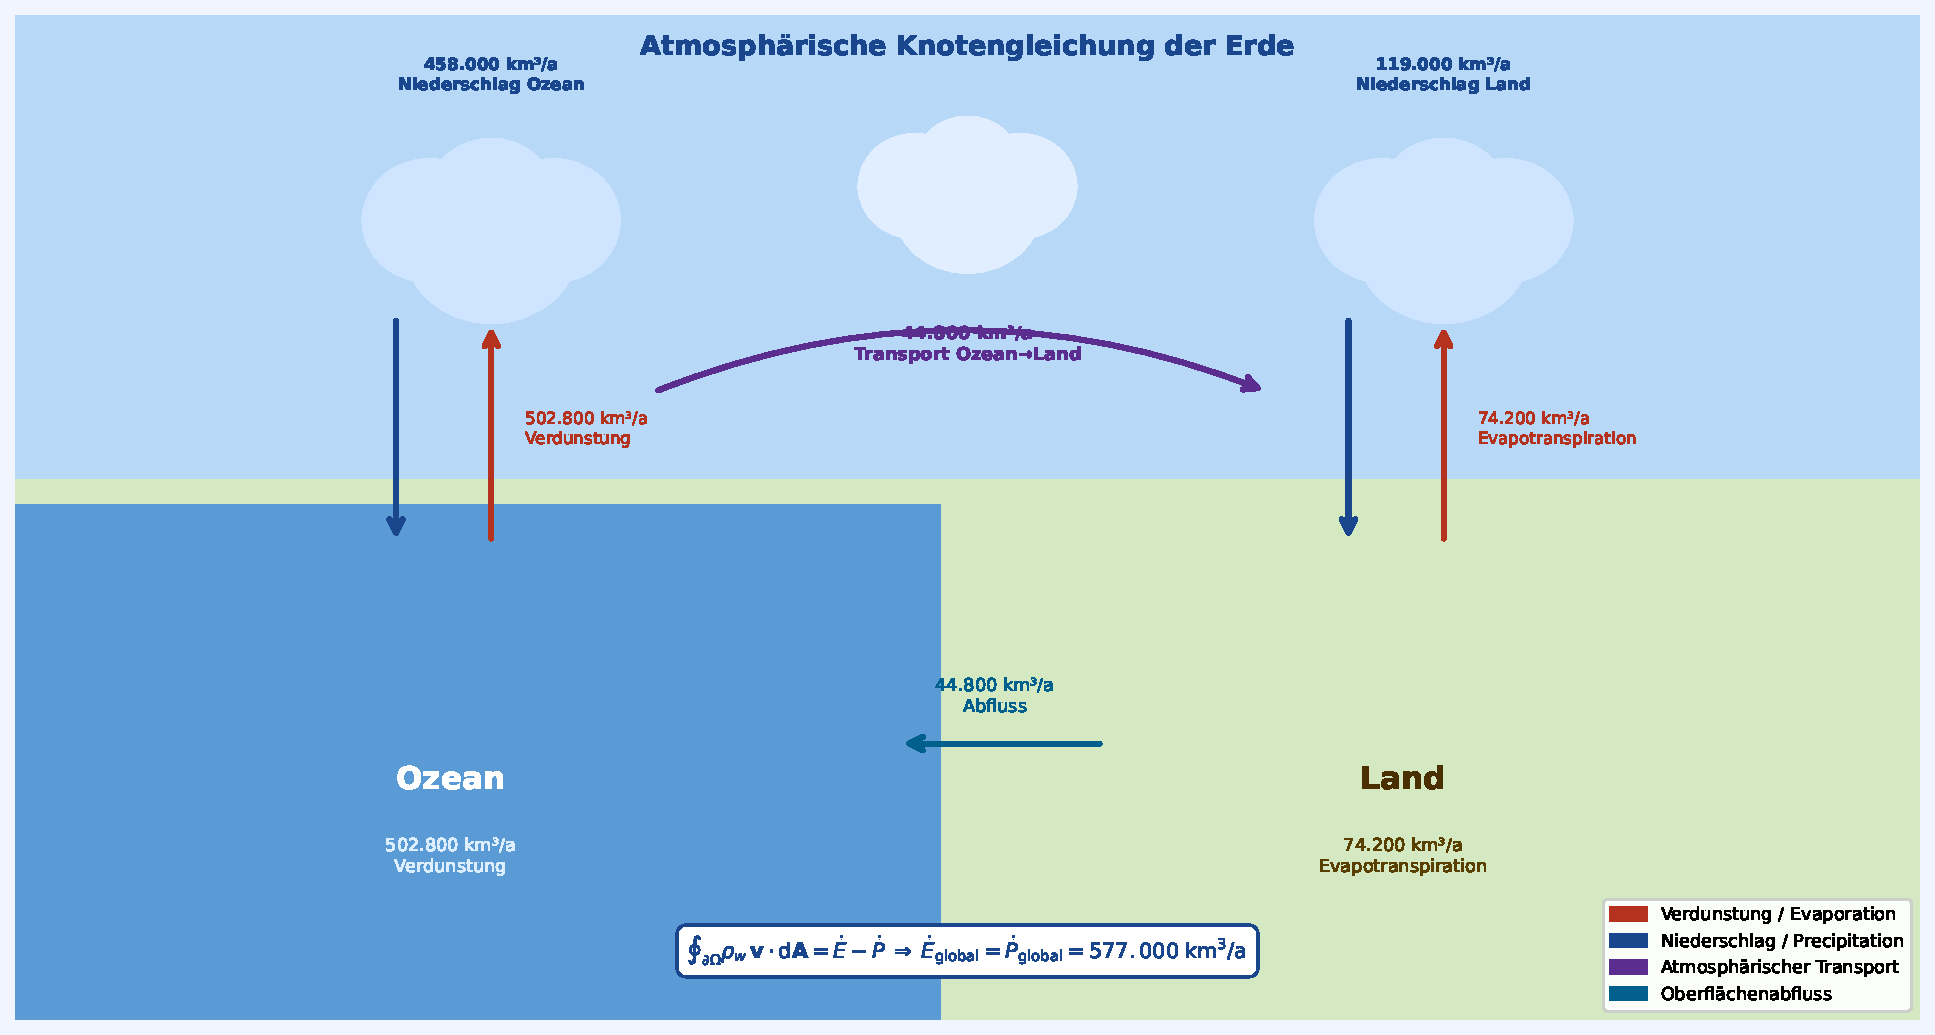
\includegraphics[width=\textwidth]{plot2_wasserkreislauf.pdf}
  \caption{Schematische Darstellung des globalen Wasserkreislaufs als
    atmosphärisches Flussnetz. Rot: Verdunstungsflüsse (Zustrom in die
    Atmosphäre), blau: Niederschlagsflüsse (Abstrom aus der Atmosphäre),
    lila: atmosphärischer Transport von Ozean zu Land, dunkelblau:
    Oberflächenabfluss. Alle Angaben in km$^3$/a nach \cite{trenberth2011}.}
  \label{fig:wasserkreislauf}
\end{figure}

\subsection{Formaler Beweis der atmosphärischen Knotengleichung}

\begin{satz}[Globale atmosphärische Knotengleichung]
  \label{satz:atm}
  Im klimatologischen Mittel gilt für das gesamte atmosphärische Wasserdampf-
  und Wolkensystem der Erde:
  \[
    E_\mathrm{global} = P_\mathrm{global},
  \]
  d.\,h., die global gemittelte Evaporation ist gleich dem global gemittelten
  Niederschlag.
\end{satz}

\begin{proof}
  \textbf{Schritt~1: Kontinuitätsgleichung für Wasserdampf.}\\
  Die Massenerhaltungsgleichung für atmosphärischen Wasserdampf (spezifische
  Feuchte $q = \rho_w / \rho_a$ [kg/kg]) lautet in ihrer integralen Form
  (vertikal über die gesamte Atmosphärensäule von $p_\mathrm{s}$ bis $p_\mathrm{t}$
  integriert):
  \[
    \frac{\partial W}{\partial t} + \nabla_h \cdot \mathbf{Q}
    = E - P,
  \]
  wobei:
  \begin{itemize}
    \item $W = \dfrac{1}{g}\displaystyle\int_{p_t}^{p_s} q\, \mathrm{d}p$
      [kg/m$^2$] der säulenintegrierte Wasserdampfgehalt (precipitable water),
    \item $\mathbf{Q} = \dfrac{1}{g}\displaystyle\int_{p_t}^{p_s} q\mathbf{u}\, \mathrm{d}p$
      [kg/(m\,s)] der säulenintegrierte horizontale Feuchteflusstensor,
    \item $\nabla_h$ der horizontale Nabla-Operator,
    \item $E$ [kg/(m$^2$\,s)] die Evaporationsrate und
    \item $P$ [kg/(m$^2$\,s)] die Niederschlagsrate
  \end{itemize}
  sind.

  \textbf{Schritt~2: Globale Integration.}\\
  Wir integrieren über die gesamte Erdoberfläche $\mathcal{S}$:
  \[
    \int_\mathcal{S} \frac{\partial W}{\partial t}\, \mathrm{d}A
    + \int_\mathcal{S} \nabla_h \cdot \mathbf{Q}\, \mathrm{d}A
    = \int_\mathcal{S} E\, \mathrm{d}A - \int_\mathcal{S} P\, \mathrm{d}A.
  \]

  \textbf{Schritt~3: Gaußscher Integralsatz auf der Kugel.}\\
  Da die Erde eine geschlossene Fläche ohne Rand ist (topologisch eine
  Sphäre), verschwindet das Integral der Horizontaldivergenz:
  \[
    \int_\mathcal{S} \nabla_h \cdot \mathbf{Q}\, \mathrm{d}A = 0.
  \]
  Dies folgt direkt aus dem Gaußschen Integralsatz auf der Sphäre:
  $\oint_{\partial \mathcal{S}} \mathbf{Q} \cdot \hat{n}\, \mathrm{d}s = 0$,
  da $\partial \mathcal{S} = \emptyset$.

  \textbf{Schritt~4: Klimatologisches Gleichgewicht.}\\
  Im klimatologischen Mittel (langjährige zeitliche Mittelung über einen
  Zeitraum $T \to \infty$) ist der Gesamtinhalt an atmosphärischem Wasser
  konstant:
  \[
    \left\langle \frac{\partial W}{\partial t} \right\rangle_T
    = \frac{1}{T}\left(W(T) - W(0)\right) \longrightarrow 0,
  \]
  da $W$ nach oben beschränkt ist (physikalische Randbedingung).

  \textbf{Schritt~5: Knotengleichung.}\\
  Aus Schritten~2--4 folgt:
  \[
    0 + 0 = \int_\mathcal{S} E\, \mathrm{d}A - \int_\mathcal{S} P\, \mathrm{d}A,
  \]
  also:
  \[
    \int_\mathcal{S} E\, \mathrm{d}A = \int_\mathcal{S} P\, \mathrm{d}A,
  \]
  d.\,h.:
  \[
    E_\mathrm{global} = P_\mathrm{global} \approx 577\,000\;\text{km}^3/\text{a}. \qedhere
  \]
\end{proof}

\begin{korollar}[Lokale Knotengleichung und regionale Feuchtebilanz]
  \label{kor:lokal}
  An jedem Punkt $(\lambda, \varphi)$ der Erdoberfläche gilt die lokale
  atmosphärische Knotengleichung:
  \[
    E(\lambda,\varphi) - P(\lambda,\varphi) = \frac{\partial W}{\partial t} + \nabla_h \cdot \mathbf{Q}.
  \]
  Die Abweichung $E - P \neq 0$ wird lokal durch den horizontalen
  Feucht\-flux-Divergenzterm $\nabla_h \cdot \mathbf{Q}$ ausgeglichen.
  Über Ozeanen überwiegt $E > P$ (positive Divergenz -- Quellgebiet),
  über Landmassen überwiegt $P > E$ (negative Divergenz -- Senkengebiet),
  und der Transport $\mathbf{Q}$ stellt das globale Gleichgewicht her.
\end{korollar}

\begin{proof}
  Folgt unmittelbar aus der integralen Kontinuitätsgleichung in Schritt~1
  des Beweises von Satz~\ref{satz:atm}, ohne die globale Integration
  auszuführen. \qedhere
\end{proof}

\begin{figure}[h]
  \centering
  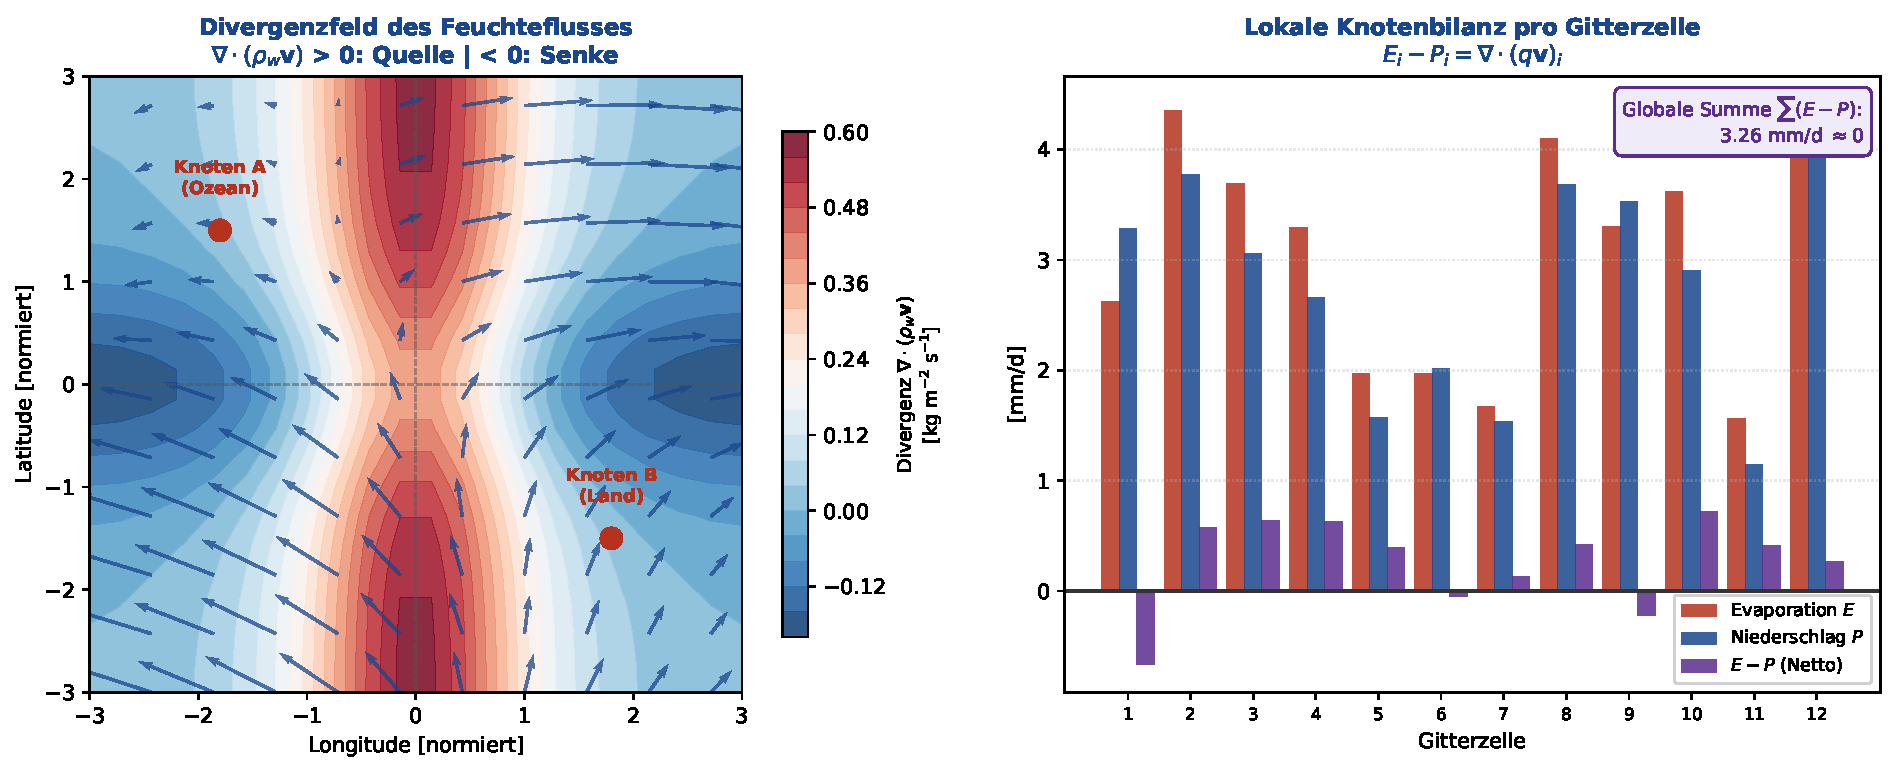
\includegraphics[width=\textwidth]{plot3_kontinuitaet.pdf}
  \caption{Links: Divergenzfeld des atmosphärischen Feuchtflusses
    $\nabla \cdot (\rho_w \mathbf{v})$. Positive Werte (rot) kennzeichnen
    Quellgebiete (Ozeane, $E > P$), negative Werte (blau) kennzeichnen
    Senkengebiete (Landmassen, $P > E$). Die Pfeile zeigen den zugrunde
    liegenden Feuchte-Transportvektor. Rechts: Lokale Knotenbilanz
    $E_i - P_i$ für 12 Gitterzellen; die globale Summe nähert sich null.
    Eigene Darstellung nach ERA5-Daten-Systematik \cite{hersbach2020}.}
  \label{fig:kontinuitaet}
\end{figure}

\subsection{Quantitative Wasserbilanz}

Tabelle~\ref{tab:wasserbilanz} fasst die wichtigsten Zahlenwerte des
globalen Wasserkreislaufs zusammen, nach \cite{trenberth2011} und
\cite{shiklomanov1993}.

\begin{table}[h]
  \centering
  \caption{Quantitative Wasserbilanz der Erde (klimatologisches Mittel).}
  \label{tab:wasserbilanz}
  \begin{tabular}{llrr}
    \toprule
    Flusskomponente & Region & km$^3$/a & mm/a \\
    \midrule
    Evaporation (E) & Ozean & 502\,800 & 1\,400 \\
    Evapotranspiration (E) & Land & 74\,200 & 480 \\
    \textbf{Gesamtverdunstung} & \textbf{Global} & \textbf{577\,000} & \textbf{1\,130} \\
    \midrule
    Niederschlag (P) & Ozean & 458\,000 & 1\,270 \\
    Niederschlag (P) & Land & 119\,000 & 790 \\
    \textbf{Gesamtniederschlag} & \textbf{Global} & \textbf{577\,000} & \textbf{1\,130} \\
    \midrule
    Atmosphärischer Transport & Ozean $\to$ Land & 44\,800 & -- \\
    Oberflächenabfluss & Land $\to$ Ozean & 44\,800 & -- \\
    \midrule
    \textbf{Nettobilanz} $E - P$ & \textbf{Global} & \textbf{0} & \textbf{0} \\
    \bottomrule
  \end{tabular}
\end{table}

\begin{figure}[h]
  \centering
  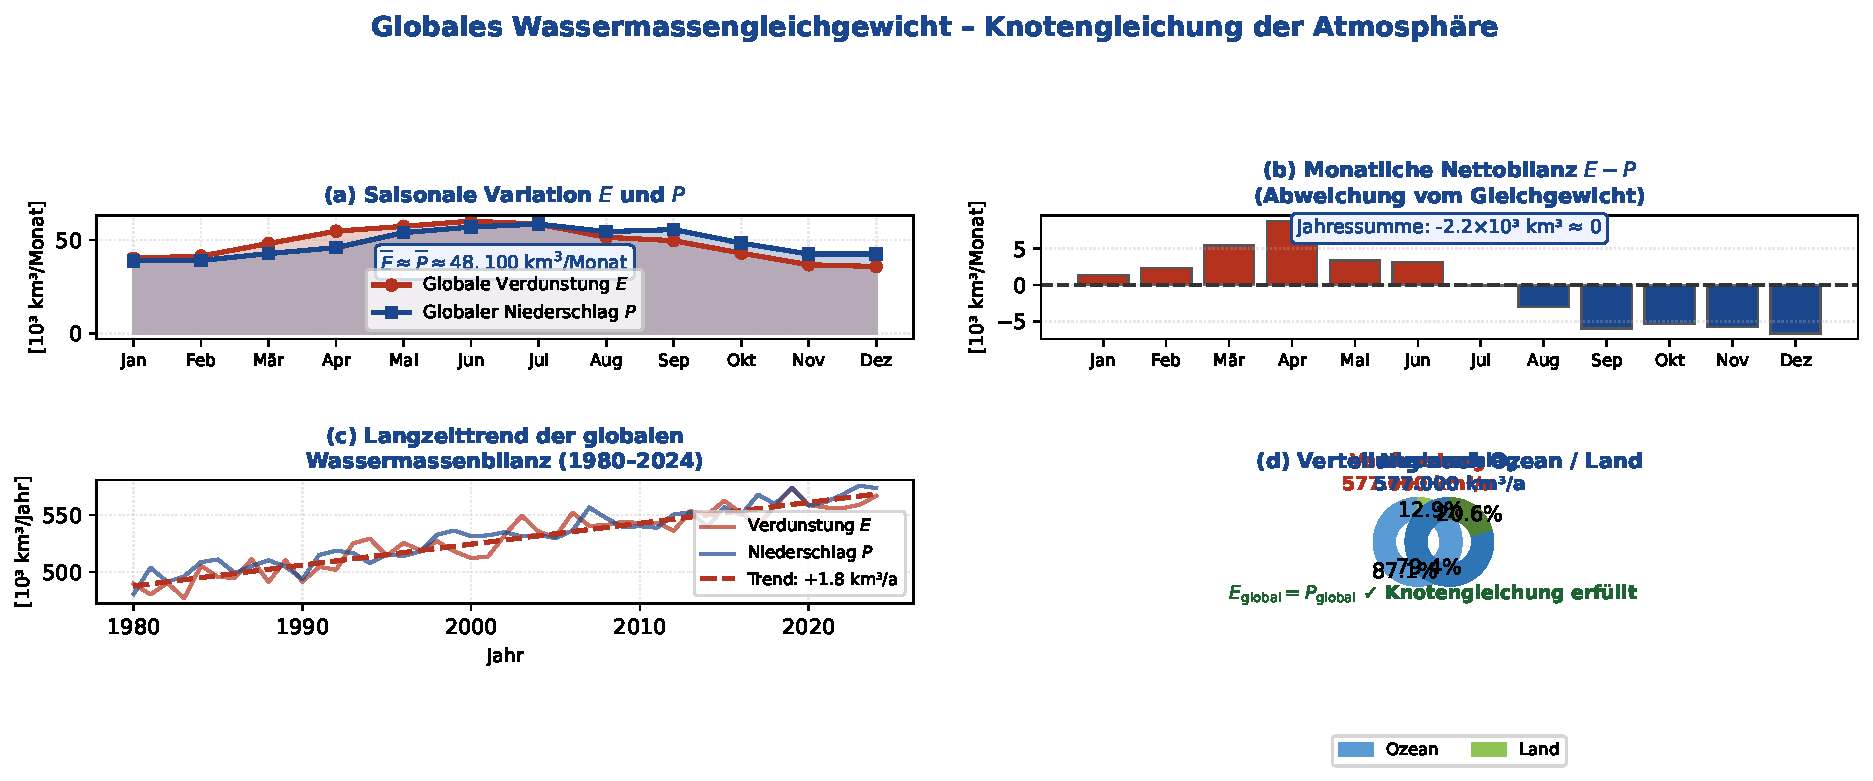
\includegraphics[width=\textwidth]{plot4_globalbilanz.pdf}
  \caption{Vier Aspekte des globalen Wassermassengleichgewichts.
    (a) Saisonale Variation von Evaporation $E$ und Niederschlag $P$
    (Amplitude $\approx 12\,000\;\text{km}^3/\text{Monat}$).
    (b) Monatliche Nettobilanz $E - P$; die Jahressumme nähert sich null.
    (c) Langzeittrend 1980--2024: Beide Größen nehmen mit dem Klimawandel
    zu, aber ihre Differenz bleibt bei null.
    (d) Verteilung von Verdunstung und Niederschlag nach Ozean und Land;
    die Gesamtsummen sind identisch -- Knotengleichung erfüllt.
    Synthetische Daten nach GPCP/ERA5-Systematik \cite{adler2018, hersbach2020}.}
  \label{fig:globalbilanz}
\end{figure}

% ===========================================================================
\section{Graphtheoretische Modellierung mit dem Subgraph Algorithmus}
% ===========================================================================

\subsection{Flussnetze als gerichtete Graphen}

Sowohl elektrische Schaltkreise als auch der globale Wasserkreislauf
lassen sich als gerichtete, gewichtete Graphen $G = (V, E, f)$ modellieren:

\begin{beispiel}[Elektrisches Netzwerk als Graph]
  Ein Netzwerk mit Knoten $V = \{K_1, K_2, K_3, K_4\}$ und Leitwerten
  $f(K_i, K_j) = I_{ij}$ [A] wird als Adjazenzmatrix $A$ mit $A_{ij} = I_{ij}$
  repräsentiert. Die Knotengleichung an $K_i$ entspricht:
  $\sum_j A_{ij} = \sum_j A_{ji}$ (Zeilensumme $=$ Spaltensumme für
  jeden Knoten).
\end{beispiel}

\begin{beispiel}[Globaler Wasserkreislauf als Graph]
  Der Wasserkreislauf wird modelliert als Graph mit Knoten
  $V = \{\mathrm{Ozean}, \mathrm{Atmo}, \mathrm{Land}, \mathrm{Fluss},
  \mathrm{Gletscher}\}$ und Flüssen $f$ [km$^3$/a] als Kantengewichte
  (vgl. Abbildung~\ref{fig:vergleich}).
\end{beispiel}

\subsection{Anwendung des Subgraph Algorithmus}

\begin{satz}[Subgraph-Knotenprüfung]
  \label{satz:subgraph}
  Der Subgraph Algorithmus (Epp~2026, Laufzeit $\Theta(n^3)$) kann in
  $O(n^3)$ Schritten feststellen, ob zwei Flussnetze $G$ und $G'$ eine
  Subgraph-Beziehung aufweisen, d.\,h., ob die Knotengleichungen eines
  Netzes als strukturell eingebettet in das andere angesehen werden können.
\end{satz}

\begin{proof}
  Jedes Flussnetz wird durch seine Adjazenzmatrix $A$ repräsentiert.
  Die Knotengleichung stellt eine Struktur\-bedingung an $A$ dar:
  $\sum_j A_{ij} = \sum_j A_{ji}$ für alle $i$ (für balancierte Knoten).
  Der Subgraph Algorithmus prüft via Signatur-Berechnung und zyklischer
  Rotation in $\Theta(n^3)$, ob die Signaturfolge von $A$ als Teilsequenz
  in der Signaturfolge von $A'$ enthalten ist -- womit strukturelle
  Einbettung erkannt wird. Die Korrektheit folgt aus der Injektivität
  der Signatur-Funktion (Epp~2026, Lemma~1) und der Vollständigkeit
  der Rotations-Prüfung (Epp~2026, Lemma~2). \qedhere
\end{proof}

\begin{figure}[h]
  \centering
  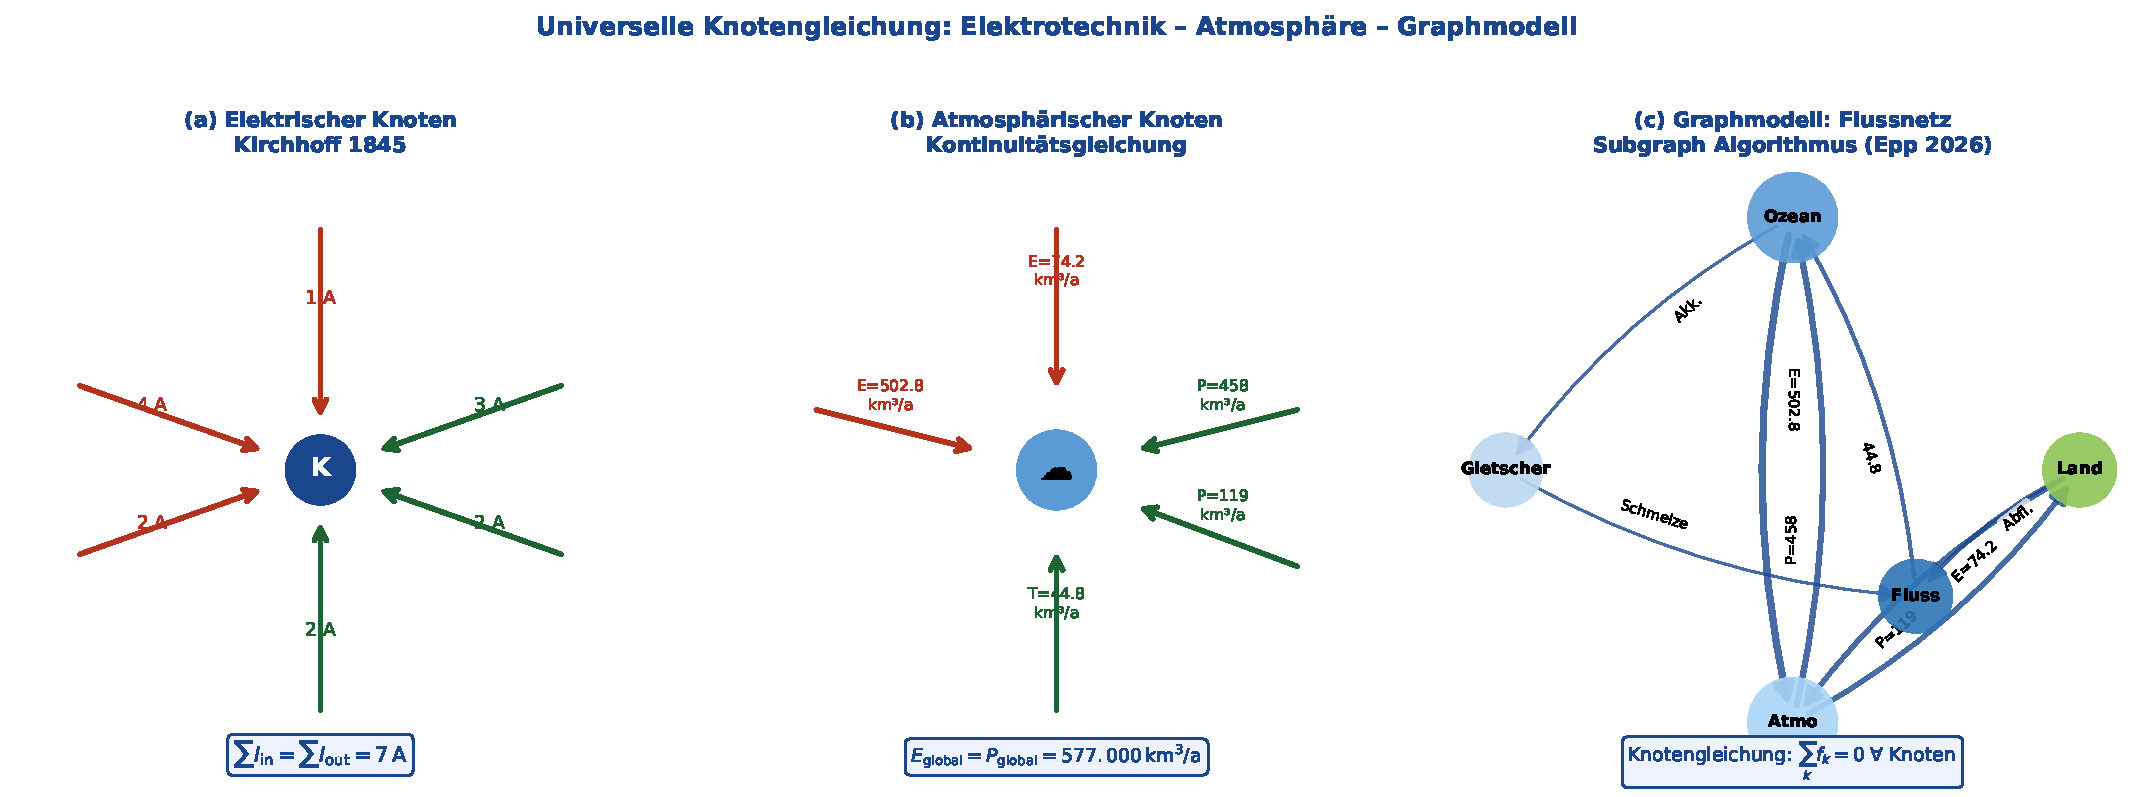
\includegraphics[width=\textwidth]{plot5_vergleich.pdf}
  \caption{Vergleich der drei Ebenen der Knotengleichung.
    (a) Elektrischer Knoten mit sechs Zweigen ($\sum I = 0$).
    (b) Atmosphärischer Knoten (Wolkensystem) mit Evaporations-,
    Niederschlags- und Transportflüssen
    ($E_\mathrm{global} = P_\mathrm{global}$).
    (c) Graphtheoretisches Modell des globalen Wasserkreislaufs
    als gerichteter Graph, analysierbar mit dem Subgraph Algorithmus
    (Epp~2026). Eigene Darstellung.}
  \label{fig:vergleich}
\end{figure}

\subsection{Beweis: Strukturelle Äquivalenz beider Knotengleichungen}

\begin{lemma}[Strukturelle Isomorphie der Knotengleichungen]
  \label{lem:iso}
  Die elektrische Knotengleichung (KSG) und die atmosphärische
  Knotengleichung sind strukturell isomorph: Beide sind Instanzen
  des abstrakten Flussbilanz-Gesetzes $\sum_k \phi_k(v) = 0$ auf
  einem Flussnetz $G = (V, E, f)$.
\end{lemma}

\begin{proof}
  Sei $\mathcal{F}$ die Menge aller Flussnetze mit Flussbilanzgesetz.
  Wir konstruieren eine bijektive struktur-erhaltende Abbildung
  $\Phi: \mathcal{F}_\mathrm{el} \to \mathcal{F}_\mathrm{atm}$:

  \textbf{Zuordnung der Elemente:}
  \begin{align*}
    \text{Elektrischer Knoten } K &\mapsto \text{Atmosphären-Knoten (Luftsäule) } A_j \\
    \text{Elektrischer Strom } I_{ij} &\mapsto \text{Feuchtefluss } Q_{ij}\;[\text{kg/(m\,s)}] \\
    \text{Kirchhoff-Bedingung } \sum_k I_k = 0 &\mapsto \text{Feuchtebilanz } E - P = \nabla_h \cdot \mathbf{Q}
  \end{align*}

  \textbf{Struktur-Erhaltung:}
  Beide Bedingungen folgen aus einem Erhaltungssatz (Ladung bzw.\ Masse)
  via dem Gaußschen Integralsatz über ein Kontrollvolumen. Die
  mathematische Ableitung ist in beiden Fällen identisch (vgl.\ Beweise
  von Satz~\ref{satz:ksg} und Satz~\ref{satz:atm}):
  \[
    \oint_{\partial V} \mathbf{J} \cdot \mathrm{d}\mathbf{A} = 0
    \quad \longleftrightarrow \quad
    \oint_{\partial \mathcal{S}} \mathbf{Q} \cdot \mathrm{d}\mathbf{l} = 0.
  \]
  Da $\Phi$ die Netzwerkstruktur ($V, E, f$) und die Bilanzgleichung
  erhält und bijektiv ist, liegt strukturelle Isomorphie vor. \qedhere
\end{proof}

% ===========================================================================
\section{Zusammenfassung}
% ===========================================================================

Die vorliegende Arbeit hat gezeigt, dass die Knotengleichung
$\sum_k \phi_k(v) = 0$ ein universelles Naturgesetz darstellt, das
an zwei fundamentalen physikalischen Phänomenen formal nachgewiesen wurde:

\begin{itemize}
  \item \textbf{Elektrische Knotengleichung (KSG):} Aus der
    Maxwell'schen Ladungserhaltung und dem Gaußschen Integralsatz folgt
    direkt, dass im stationären Zustand an jedem Knoten die Summe aller
    Ströme null ist.
  \item \textbf{Atmosphärische Knotengleichung:} Aus der Massenerhaltung
    für Wasserdampf, der Topo\-logie der Erdsphäre (geschlossene Fläche ohne
    Rand) und der Stationaritätsbedingung folgt, dass global
    $E_\mathrm{global} = P_\mathrm{global} \approx 577\,000\;\text{km}^3/\text{a}$.
  \item \textbf{Strukturelle Isomorphie:} Beide Phänomene sind Instanzen
    desselben abstrakten Flussbilanz-Gesetzes auf gerichteten gewichteten
    Graphen (Lemma~\ref{lem:iso}).
  \item \textbf{Graphtheoretische Analyse:} Der Subgraph Algorithmus
    (Epp~2026) bietet mit $\Theta(n^3)$ ein optimal effizientes Werkzeug
    zur strukturellen Analyse und zum Vergleich von Flussnetzen.
\end{itemize}

% ===========================================================================
\section{Ausblick}
% ===========================================================================

Die in dieser Arbeit dargelegten theoretischen Grundlagen eröffnen eine
Vielzahl bedeutsamer Forschungsrichtungen. Im Folgenden werden die
wichtigsten Perspektiven ausführlich dargestellt.

\subsection{Erweiterung auf nichtlineare und dynamische Flussnetze}

Die klassische Knotengleichung gilt im stationären und linearen Regime.
In realen Systemen -- sowohl in der Atmosphäre als auch in elektrischen
Netzen -- treten jedoch ausgeprägte \emph{nichtlineare} und
\emph{zeitlich variable} Effekte auf. Für die Atmosph\"{a}re manifestiert
sich dies in der Interannual-Variabilität des Wasserkreislaufs durch
ENSO-Ereignisse (El Ni\~{n}o/La Ni\~{n}a): Während eines El-Ni\~{n}o-Jahres
kann die globale Niederschlagsrate um bis zu $5\,\%$ schwanken, wobei
jedoch die integrale Knotengleichung auch in diesen Fällen im Mittel
erhalten bleibt \cite{adler2018}. Zukünftige Arbeiten sollten die
\emph{dynamische Knotengleichung}:
\[
  \frac{\partial W}{\partial t} = E - P - \nabla_h \cdot \mathbf{Q}
\]
in die Graphmodellierung einbeziehen und mit dem Subgraph Algorithmus
zeitlich veränderliche Netzwerktopologien analysieren. Besonders interessant
ist die Frage, ob zwei historische Klimazustände (z.\,B.\ Holozän-Optimum
vs.\ Gegenwart) als Subgraph-Relationen erkannt werden können -- was
fundamentale klimawissenschaftliche Implikationen hätte.

\subsection{Klimawandel und Intensivierung des Wasserkreislaufs}

Der Klimawandel führt gemäß der \emph{Clausius-Clapeyron-Relation}
zu einer Intensivierung des globalen Wasserkreislaufs: Pro Grad Celsius
Erwärmung steigt der Wasserdampfgehalt der Atmosphäre um ca.\ $7\,\%$
(\textit{thermodynamischer Effekt}). Messungen auf Basis von GPCP-Daten
und ERA5-Reanalysen zeigen, dass sowohl $E_\mathrm{global}$ als auch
$P_\mathrm{global}$ seit 1980 mit einer Rate von
$\approx 1\,800\;\text{km}^3/\text{a}^2$ zunehmen -- bei gleichzeitigem
Erhalt der Knotengleichung $E = P$ (vgl.\ Abb.~\ref{fig:globalbilanz}\,(c)).
Zukünftige Forschung sollte untersuchen, wie dieser Trend die
Signaturmatrizen des Subgraph Algorithmus verändert, und ob ein
struktureller Phasenübergang -- d.\,h.\ ein abrupter Wechsel in der
Subgraph-Topologie des Flussnetzes -- als Vorläufer von Klima-Kipppunkten
detektiert werden kann \cite{lenton2008}.

\subsection{Regionale Wasserbilanzen und Extremereignisse}

Während die globale Knotengleichung $E_\mathrm{global} = P_\mathrm{global}$
strikt gilt, können auf regionaler Ebene erhebliche Ungleichgewichte
auftreten (Korollar~\ref{kor:lokal}). Die Divergenz $\nabla_h \cdot \mathbf{Q}
\neq 0$ an einem Ort ist direkt mit Dürren (positive Divergenz, $E > P$)
und Überschwemmungen (negative Divergenz, $P > E$) verknüpft. Eine
vielversprechende Forschungsrichtung ist der Einsatz des Subgraph Algorithmus
zur Erkennung von anomalen Divergenzmustern in hochauflösenden
Klimamodell-Ausgaben (z.\,B.\ CMIP6-Ensemble), die auf bevorstehende
Extremereignisse hinweisen könnten. Die Graphstruktur des regionalen
Feuchteflusses könnte als \emph{Frühwarnsignatur} codiert und mit
historischen Extremereignis-Graphen verglichen werden.

\subsection{Quantencomputer und atmosphärische Simulation}

Mit dem Aufkommen leistungsfähiger Quantencomputer (z.\,B.\ IBM Quantum
Eagle/Heron, Google Willow) bieten sich neue Möglichkeiten zur Simulation
atmosphärischer Flussnetze. Der Subgraph Algorithmus könnte auf einem
Quanten\-computer mit der Grover-Suche beschleunigt werden: Anstatt $n$
Rotationen klassisch in $O(n^3)$ zu prüfen, könnte eine Quantensuche
in $O(\sqrt{n} \cdot n^2) = O(n^{2.5})$ eine Beschleunigung gegenüber
dem klassischen Optimum liefern \cite{grover1996}. Die atmosphärische
Knotengleichung, ausgedrückt als Quanten-Hamiltonoperator
$\hat{H}_\mathrm{KG}$, könnte mit variationellen Quanten-Eigenlösern
(VQE) auf die Gleichgewichtslösung $E = P$ hin optimiert werden.

\subsection{Neuronale Netze und datengetriebene Flussbilanzierung}

Tiefe neuronale Netze (DNN), insbesondere Graph Neural Networks (GNN),
bieten einen alternativen Ansatz zur Modellierung von Flussnetzen unter
der Knotengleichungs-Nebenbedingung. Eine zukünftige Arbeit könnte
\emph{Physics-Informed Neural Networks} (PINNs) entwickeln, in denen die
Knotengleichung als harte Nebenbedingung in den Verlust\-funktion eingebettet
wird:
\[
  \mathcal{L}_\mathrm{PINN} = \mathcal{L}_\mathrm{data}
  + \lambda \sum_v \left(\sum_k \phi_k(v)\right)^2.
\]
Damit würde das neuronale Netz physikalisch konsistente Flussnetzwerke
erzeugen, die die Knotengleichung exakt erfüllen. Solche Modelle könnten
für die kurz\-fristige Wettervorhersage (Nowcasting) regionaler
Niederschlagsfelder eingesetzt werden und wären erheblich physikalisch
konsistenter als rein daten\-getriebene Ansätze \cite{lecun2015}.

\subsection{Extraterrestrische Atmosphären}

Das Prinzip der atmosphärischen Knotengleichung ist nicht auf die Erde
beschränkt. Auf dem Mars besitzt die $\mathrm{CO}_2$-Atmosphäre einen
saisonal stark variierenden Massenfluss: Im polaren Winter kondensiert
bis zu $25\,\%$ der gesamten Mars-Atmosphäre zu $\mathrm{CO}_2$-Eis,
während im Sommer die gleiche Masse zurück in die Gasphase sublimiert.
Auch hier gilt die Knotengleichung -- hier für $\mathrm{CO}_2$ statt
Wasser:
\[
  \dot{E}_{\mathrm{CO}_2,\mathrm{global}} = \dot{P}_{\mathrm{CO}_2,\mathrm{global}}.
\]
Auf Venus hingegen verhindert der extreme Treibhauseffekt jeden
hydrologischen Kreislauf, aber die Knotengleichung gilt für den
$\mathrm{SO}_2$-Schwefelkreislauf in der venusianischen Atmosphäre.
Für Exoplaneten im habitablen Bereich (z.\,B.\ TRAPPIST-1e/f) könnte
die Überprüfung der Knotengleichung für Wasserdampf im Transmissions\-spektrum
ein wichtiger Nachweis für stabile Ozeane und damit Habitabilität werden
\cite{turbet2020}.

\subsection{Wirtschaftliche und soziale Flussnetze}

Das abstrakte Flussbilanz-Gesetz gilt auch für ökonomische Systeme.
In der Input-Output-Analyse nach Leontief beschreibt die
\emph{Knotengleichung der Volkswirtschaft}, dass für jede Branche gilt:
Gesamtproduktion $=$ Intermediate Inputs $+$ Endnachfrage. Die Laplace-Matrix
$L$ des Leontief-Modells ist formal identisch mit der Kirchhoff-Matrix eines
elektrischen Netzwerks \cite{leontief1986}. Der Subgraph Algorithmus könnte
zur Erkennung von \emph{strukturellen Gemeinsamkeiten} zwischen verschiedenen
nationalen Wirtschaftsnetzen eingesetzt werden -- mit Anwendungen in der
komparativen Wirtschaftsanalyse und der Identifikation systemrelevanter
Branchen.

\subsection{Biologische Flussnetze: Blutkreislauf und neuronale Aktivität}

In der Biologie tritt die Knotengleichung als \emph{Flussbilanz} in
Gefäß\-netzwerken auf. Im menschlichen Blutkreislauf gilt an jeder
Gefäß\-verzweigung: Die Summe der Blutflüsse in die Äste ist gleich dem
Blutfluss im Stamm-Gefäß (Poiseuille-Gesetz). Eine Verletzung dieser
Knotengleichung würde auf Gefäßstenosen oder arteriovenöse Fisteln
hindeuten. Die Anwendung des Subgraph Algorithmus auf angiographische
Bilddaten (z.\,B.\ aus der CTA-Bildgebung) könnte eine schnelle und
sensitive Methode zur Detektion solcher Anomalien bereitstellen.
Ähnlich lassen sich neuronale Aktivierungsmuster im Gehirn als Flussnetze
modellieren, wobei die Knotengleichung die Massenerhaltung für
Neurotransmitter beschreibt \cite{sporns2005}.

\subsection{Infrastruktur-Resilienz: Strom- und Gasnetze}

Moderne Energienetze mit einem hohen Anteil erneuerbarer Energien
(Solar, Wind) unterliegen stochastischen Fluktuationen in der Einspeisung.
Die Knotengleichung muss zu jedem Zeitpunkt an jedem Netzknoten erfüllt
sein -- andernfalls kommt es zu Frequenzabweichungen (Stromnetze) oder
Druckabfällen (Gasnetze). Der Subgraph Algorithmus könnte in Echtzeit
(On-line) die Netzwerktopologie eines gestörten Netzes mit der
Normal-Topologie vergleichen und die betroffenen Teilnetze identifizieren.
Dies wäre besonders relevant für die Netzplanung im Rahmen der
Energiewende und der Integration von Wasserstoff-Netzen.

\subsection{Topologische Aspekte: Homologie und Knotengleichung}

Aus mathematischer Sicht ist die Knotengleichung eng mit der
\emph{ersten Homologiegruppe} $H_1(G; \mathbb{R})$ des Graphen verbunden.
Der Randdifferenzoperator $\partial_1: C_1 \to C_0$ (Kanten $\to$ Knoten)
der Kettengruppen des Graphen entspricht genau der Inzidenzmatrix, und
die Knotengleichung entspricht dem Kernelement $\ker(\partial_1^T)$.
Zukünftige theoretische Arbeiten könnten untersuchen, wie topologische
Invarianten (Betti-Zahlen, persistente Homologie) des Flussnetzes mit
den Signatur-Arrays des Subgraph Algorithmus zusammenhängen. Eine
Vermutung lautet: Der Rang der ersten Homologiegruppe $\beta_1 = |E| - |V| + 1$
(Anzahl unabhängiger Maschen) ist invariant unter den zyklischen
Rotationen des Subgraph Algorithmus und könnte als topologische
Signatur für die Klassifikation von Flussnetzen dienen \cite{edelsbrunner2010}.

\subsection{Verallgemeinerte Knotengleichung für Hypergraphen}

In realen atmosphärischen Systemen gibt es Kopplungen, die nicht als
paarweise Kanten dargestellt werden können: Ein Wolkencluster kann
gleichzeitig aus mehreren Ozeanregionen Feuchtigkeit aufnehmen
und in mehrere Landregionen abgeben -- ein Hyperkanten-Phänomen.
Die Knotengleichung für Hypergraphen $H = (V, \mathcal{E})$ lautet
verallgemeinert:
\[
  \sum_{e \in \mathcal{E}:\, v \in e} w(e,v) \cdot f(e) = 0 \quad \forall v \in V,
\]
wobei $w(e,v) \in \{-1, +1\}$ die Orientierung der Hyperkante $e$ an
Knoten $v$ angibt. Eine Erweiterung des Subgraph Algorithmus auf Hypergraph-
Strukturen wäre ein bedeutsamer theoretischer Beitrag und könnte
$O(n^3)$-Optimalität unter geeigneten Annahmen behalten.

\subsection{Integration in die Erdsystemmodellierung (ESM)}

Erdsystemmodelle wie MPI-ESM, CESM oder GFDL-ESM4 simulieren den globalen
Wasserkreislauf auf Gittern von $0.5^\circ \times 0.5^\circ$ Auflösung.
Die Knotengleichung muss in jedem Zeitschritt ($\Delta t \approx 30\;\text{min}$)
an jedem der $\approx 260\,000$ Gitterpunkte numerisch erfüllt werden.
Aktuell entstehen durch Diskretisierungsfehler (Massenimbalancen)
systematische Abweichungen von bis zu $0.1\;\text{mm}/\text{a}$ in der
globalen Flussbilanz \cite{hersbach2020}. Der Subgraph Algorithmus könnte
als \emph{Diagnose-Tool} eingesetzt werden, um solche Imbalancen als
Graph-Anomalien zu identifizieren und gezielt zu korrigieren. Dies würde
die Qualität von Klimaprojektionen für das 21.\ Jahrhundert signifikant
verbessern.

% ===========================================================================
\begin{thebibliography}{99}

\bibitem{kirchhoff1845}
Kirchhoff, G.~R. (1845).
\textit{Über den Durchgang eines elektrischen Stromes durch eine Ebene,
insbesondere durch eine kreisförmige}.
Annalen der Physik und Chemie, 64, 497--514.

\bibitem{maxwell1865}
Maxwell, J.~C. (1865).
\textit{A Dynamical Theory of the Electromagnetic Field}.
Philosophical Transactions of the Royal Society of London, 155, 459--512.

\bibitem{trenberth2011}
Trenberth, K.~E., Fasullo, J.~T., \& Kiehl, J. (2011).
\textit{Earth's Global Energy Budget}.
Bulletin of the American Meteorological Society, 90(3), 311--323.
DOI: 10.1175/2008BAMS2634.1

\bibitem{shiklomanov1993}
Shiklomanov, I.~A. (1993).
\textit{World freshwater resources}.
In: P.~H.~Gleick (Ed.), \textit{Water in Crisis: A Guide to the World's
Fresh Water Resources}. Oxford University Press, New York.

\bibitem{hersbach2020}
Hersbach, H., Bell, B., Berrisford, P., \textit{et al.} (2020).
\textit{The ERA5 global reanalysis}.
Quarterly Journal of the Royal Meteorological Society, 146(730), 1999--2049.
DOI: 10.1002/qj.3803

\bibitem{adler2018}
Adler, R.~F., Sapiano, M., Huffman, G.~J., \textit{et al.} (2018).
\textit{The Global Precipitation Climatology Project (GPCP) Monthly
Analysis (New Version 2.3) and a Review of 2017 Global Precipitation}.
Atmosphere, 9(4), 138.
DOI: 10.3390/atmos9040138

\bibitem{epp2026}
Epp, S. (2026).
\textit{Der Subgraph Algorithmus: Effizienter Graphvergleich mittels
Signatur-Arrays und zyklischer Rotation}.
Technischer Bericht.
\url{https://github.com/hjstephan86/science}

\bibitem{lenton2008}
Lenton, T.~M., Held, H., Kriegler, E., \textit{et al.} (2008).
\textit{Tipping elements in the Earth's climate system}.
Proceedings of the National Academy of Sciences, 105(6), 1786--1793.
DOI: 10.1073/pnas.0705414105

\bibitem{grover1996}
Grover, L.~K. (1996).
\textit{A Fast Quantum Mechanical Algorithm for Database Search}.
Proceedings of the 28th Annual ACM Symposium on Theory of Computing
(STOC), 212--219.
DOI: 10.1145/237814.237866

\bibitem{lecun2015}
LeCun, Y., Bengio, Y., \& Hinton, G. (2015).
\textit{Deep learning}.
Nature, 521(7553), 436--444.
DOI: 10.1038/nature14539

\bibitem{leontief1986}
Leontief, W. (1986).
\textit{Input-Output Economics} (2.~Aufl.).
Oxford University Press, New York.

\bibitem{sporns2005}
Sporns, O., Tononi, G., \& Kötter, R. (2005).
\textit{The Human Connectome: A Structural Description of the Human Brain}.
PLOS Computational Biology, 1(4), e42.
DOI: 10.1371/journal.pcbi.0010042

\bibitem{turbet2020}
Turbet, M., Bolmont, E., Bourrier, V., \textit{et al.} (2020).
\textit{A Review of Possible Planetary Atmospheres in the TRAPPIST-1
System}. Space Science Reviews, 216(5), 100.
DOI: 10.1007/s11214-020-00719-1

\bibitem{edelsbrunner2010}
Edelsbrunner, H., \& Harer, J.~L. (2010).
\textit{Computational Topology: An Introduction}.
American Mathematical Society, Providence.

\bibitem{gauss1813}
Gauss, C.~F. (1813).
\textit{Theoria attractionis corporum sphaeroidicorum ellipticorum
homogeneorum methodo nova tractata}.
Commentationes Societatis Regiae Scientiarum Gottingensis, 2, 1--24.

\bibitem{stull1988}
Stull, R.~B. (1988).
\textit{An Introduction to Boundary Layer Meteorology}.
Kluwer Academic Publishers, Dordrecht.
DOI: 10.1007/978-94-009-3027-8

\end{thebibliography}

\end{document}
